\chapter{La planificación y el presupuesto}
\label{cap:PlanificacionPresupuesto}
% [Autores: María José Rodríguez Fórtiz]
% Se puede meter también un plan de contingencias: hecho

Cualquier proyecto que se precie debe indicar cómo se va a desarrollar en el tiempo, con objeto de mostrar su duración y cómo se van a ir realizando las tareas que lo componen, y cuánto va a costar, con objeto de determinar su viabilidad económica, tanto para un cliente que esté interesado en su realización como para nosotros mismos, o nuestra empresa, si somos quienes lo llevaremos a cabo. Y el proyecto de tu TFG no será menos. Por tanto, la memoria de tu trabajo deberá contener estos dos elementos. En este capítulo te damos algunos consejos sobre la elaboración de la planificación y del presupuesto de tu proyecto.


\section{Planificación temporal}
El objetivo de esta sección de la memoria de tu TFG es mostrar temporalmente cómo se van a organizar la ejecución de las diferentes tareas de tu TFG. Estas tareas ya deberán haber aparecido previamente, típicamente en la parte de la memoria dedicada a la metodología. Para ello, lo habitual es incluir un diagrama de Gantt con el cronograma final de realización del TFG. También puedes incluir el cronograma de planificación inicial y hacer una comparativa entre ambos, explicando sus diferencias y justificando los motivos de cambio.

Un \href{https://blog.ganttpro.com/en/ultimate-guide-gantt-charts/}{diagrama de Gantt} es una tabla en la que las columnas son unidades de tiempo (días, semanas o meses) y las filas son las tareas en las que se descompone el proyecto. Habitualmente las tareas se agrupan en paquetes de trabajo, según su funcionalidad o las etapas o fases del proyecto en el que éste se haya dividido. En las celdas de la tabla se marcará qué tareas se van a llevar a cabo en esas unidades de tiempo, de tal forma que tenemos información gráfica del comienzo, duración de tareas, y relación con otras. Ocasionalmente se pueden incluir vínculos entre tareas, para forzar relaciones de fin a comienzo. Por ejemplo, no puedo empezar una tarea B hasta que no haya terminado una tarea A. También puede haber tareas con ejecución intermitente. Por ejemplo, puedes poner una tarea de ``reuniones con mi tutor o tutora" que tenga asignados varias franjas temporales, como un día cada dos semanas.

En la figura \ref{fig:gantt} se muestra un ejemplo de un diagrama de Gantt básico para un proyecto.

\begin{figure}[!t]
    \centering
    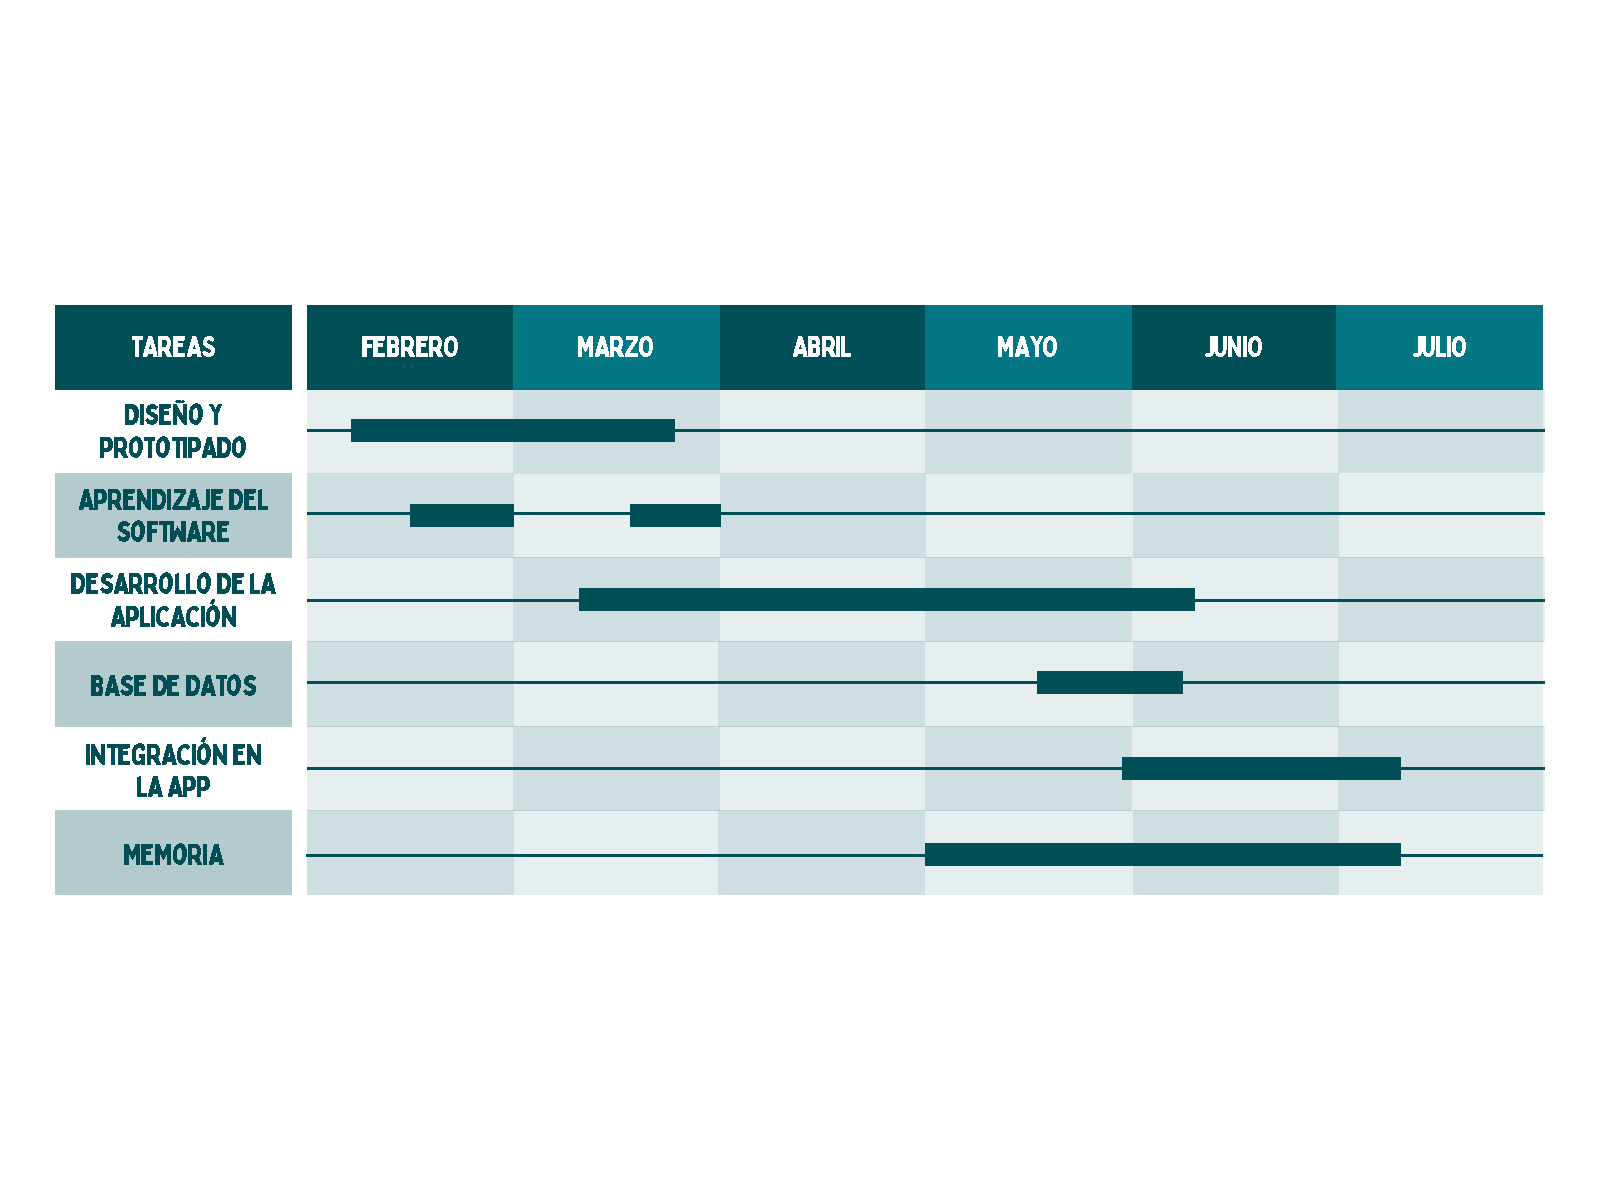
\includegraphics[width=1.0\textwidth]{images/EjemploGantt.pdf}
    \caption{Diagrama de Gantt\label{fig:gantt}}
\end{figure}

En ella se puede observar que hay seis tareas en el proyecto y que el mismo se desarrolla desde febrero a julio. A modo de ejemplo, el \textit{Diseño y prototipado} se llevará a cabo desde la segunda semana de febrero hasta la tercera semana de marzo. Además, en este diagrama hay tareas que se pueden hacer en paralelo (como el diseño y prototipado y el aprendizaje del software, entre otras). % Modificar el diagrama para poner alguna tarea secuencial para indicarlas.

El diagrama de Gantt debe incluir todas las tareas que has realizado (o vas a realizar, pues es se hace antes de comenzar a realizar las tareas) vinculadas con los objetivos del TFG. Ten en cuenta que en los objetivos de tu TFG no debe haber solo objetivos de desarrollo, sino también en muchos casos de aprendizaje, porque te plantees aprender nuevas tecnologías o conocer más del dominio de aplicación del problema que vas a abordar. También tendrás objetivos relacionados con la organización de tu trabajo como reuniones, revisiones y redacción de la memoria. Teniendo en cuenta esto, debes planificar todas las tareas necesarias para cubrir los objetivos planteados, y por ello, en el cronograma debe haber tareas de aprendizaje, de desarrollo, y de organización. En cuanto al desarrollo, si vas a seguir una metodología específica, esta tiene que verse reflejada en el cronograma. Por ejemplo, si sigues una metodología ágil con iteraciones cada dos semanas, en tu cronograma debería aparecer una tarea con duración de dos semanas por cada iteración. Si tu ciclo de vida no es iterativo sino clásico, deberían aparecer paquetes de trabajo para análisis, diseño, implementación, pruebas, etc, con tareas específicas dentro de cada uno de ellos.

Cuanto mayor sea el nivel de detalle del cronograma, mejor, ya que darás más información de las tareas y tiempo dedicados. Te aconsejamos que la unidad temporal usada en el cronograma sea semanal, aunque también puedes usar meses. 

Existen varias aplicaciones informáticas de escritorio o en línea para hacer diagramas de Gantt y gestionar cambios sobre estos. Muchas de estas herramientas permiten fijar una línea base (como una fotografía del diagrama en un momento) para comparar con cambios posteriores, de tal forma que también se pueden hacer simulaciones. Otra funcionalidad que ofrecen estas herramientas es poder asignar recursos humanos y materiales a las tareas, con costes asociados, lo cual es muy útil para hacer un presupuesto del proyecto. Algunas de estas aplicaciones te permiten trabajar en equipo haciendo un uso compartido entre varios usuarios. En tu caso podrías compartir el diagrama de planificación con la persona que te tutoriza.

A día de hoy, te podemos sugerir algunas herramientas gratuitas y sencillas para hacer y gestionar diagramas de Gantt, como son \href{https://www.ganttproject.biz/}{GanttProject}, \href{https://www.projectlibre.com/}{Project Libre}, 
 \href{https://www.monday.com}{Monday.com}, \href{https://app.clickup.com/}{Clickup}. 

También puedes hacer tu diagrama de Gantt usando \href{https://www.canva.com/}{Canva}, eligiendo una de las plantillas de este tipo que se proveen, o con una hoja de cálculo, pero en estos casos no tienes tantas facilidades para editar los cambios temporales, ni funcionalidades como las apuntadas arriba. 

Si usas un gestor de proyectos como OpenProject, Notion, Trello, Asana, etc., podrás generar automáticamente el diagrama de Gantt a partir de las tareas que hayas creado en el gestor si has definido los márgenes temporales para cada una.

Algunas recomendaciones sobre esta sección son que describas brevemente los tipos de tareas de tu diagrama y cuál es tu metodología de desarrollo para que se pueda comprender mejor. En cuanto a su visualización dentro de la memoria, debes asegurarte de que el diagrama se vea bien, para lo cual te sugerimos que lo pongas en apaisado a página completa, o que lo subdividas en varios diagramas, por ejemplo, uno por cada paquete de trabajo. El diagrama deberá formar parte de la presentación final, así que es mejor que uses colores o tramas para diferenciar mejor los tipos de tareas y para que sea más atractivo visualmente. 

\subsection{Planificación ''a posteriori``}

Una planificación, por definición, no puede ser a posteriori. Sin embargo, sí que debemos hacer el ejercicio de medir el tiempo de cada etapa del proyecto y ver cómo de real ha sido la estimación en la planificación (en la que hiciste a priori) y analizar los motivos por los que han divergido.

Con el fin de tener una representación temporal de la ejecución, debes llevar un diario de trabajo en el que anotes las tareas que has realizado cada día, el tiempo que has dedicado a cada una de ellas, y si has tenido que cambiar de tarea por algún motivo. De esta forma, al final del proyecto podrás mostrar realmente cómo has trabajado.

%OJOJOJOJOJOJOJJOJOJOJOJ ESTO NO LO VEO -> DEBE HACERSE A PRIORI
%Te será muy fácil hacer el cronograma si has sido metódico/a, apuntando cada día de trabajo en el TFG el número de horas dedicadas al TFG y a qué tarea específica las has dedicado. Solo recuerda que todo el tiempo de tu vida que dediques al proyecto debe estar reflejado en el cronograma final. 

Algunas de las aplicaciones citadas para hacer diagramas de Gantt permiten gestionar cambios sobre estos. Muchas de estas herramientas permiten fijar una línea base (como una fotografía del diagrama en un momento) para comparar con cambios posteriores, de tal forma que también se pueden hacer simulaciones. Otra funcionalidad que ofrecen estas herramientas es poder asignar recursos humanos y materiales a las tareas, con costes asociados, lo cual es muy útil para hacer un presupuesto del proyecto. Algunas de estas aplicaciones te permiten trabajar en equipo haciendo un uso compartido entre varios usuarios. En tu caso podrías compartir el diagrama de planificación con la persona que te tutoriza.

Ya te hemos recomendado algunas herramientas para medir el tiempo exacto que dedicas a cada tarea, repasa las recomendaciones generales del capítulo \ref{cap:Recomendaciones}.



\section{Plan de gestión de riesgos y contingencias}

En algunos TFG, por su temática o tecnologías usadas, o porque la persona que te tutoriza lo vea conveniente, se puede presentar un plan de gestión de riesgos. El plan es una lista de posibles riesgos que pueden surgir durante el desarrollo del TFG, cada uno de ellos con acciones para evitarlos y/o mitigarlos. 

La lista de riesgos suele priorizarse según su impacto en el proyecto. Para ello, hay que hacer un estudio previo en el que valoremos si la ocurrencia del riesgo afecta al alcance del TFG (cambios en requisitos), al tiempo (retrasos, cambio de orden y tiempo asignado a tareas), al coste (incremento de gastos), a los recursos (cambios en tecnología usada), etc. Una vez valorado esto, asignaremos más prioridad a aquellos que tengan mayor impacto. 

Teniendo en cuenta el impacto de cada riesgo, lo siguiente es planificar una acción de prevención para evitar que ocurra, si es posible. Se deben planificar acciones de mitigación si no podemos evitar que el riesgo ocurra o si el plan de prevención fallara.

Por ejemplo, un riesgo podría ser que la tecnología a usar para el desarrollo del TFG sea muy nueva, lo que conlleva que no haya apenas manuales de uso y poca gente la conozca, así que no podrás tener mucha ayuda en foros, y  si tienes algún problema con ella puede que no puedas seguir adelante y te quedes bloqueado. El impacto de ese riesgo podría afectar al alcance del proyecto, pero también al tiempo y por supuesto a los recursos. Como plan de prevención, podrías apuntarte a un curso de formación existente (aunque incremente los costes del proyecto), y como plan de mitigación, la acción propuesta podría ser dejar el uso de esa tecnología solo para una parte del desarrollo menos importante, no para todo, de tal forma que no se vea afectado el proyecto completo.

Tienes una lista de diversos tipos de riesgos y más información sobre el plan de gestión de riesgos en el capítulo de Estimación de riesgos, de \cite{guerin2018gestion}, disponible en línea en la biblioteca de la UGR.

Una vez planteado el plan de mitigación, durante el proyecto debe revisarse para decidir si se realiza alguna de las acciones previstas y en esta sección de la memoria, explicar con detalle qué acciones se han realizado y sus resultados, incluyendo comentarios sobre los costes asociados.

Si vas a incluir un plan de gestión de riesgos, consensúa con la persona que te tutoriza en qué capítulo incluirlo, ya que una opción es que sea una sección del capítulo de la propuesta, para que esté más cercano a la explicación de  cómo se han gestionado los riesgos durante el desarrollo.

\section{Presupuesto}

Con esta sección se indica al lector de la memoria cuál sería el coste de desarrollo del proyecto realizado dentro del TFG en el caso de que este proyecto se ejecutara en la vida real. Esta sección ayuda al lector valorar el tiempo dedicado por tu parte al proyecto, tus decisiones respecto a la tecnología elegida, y el coste de todo ello. Como ingeniero, debes demostrar que sabes hacer un proyecto coherente  y sensato, buscando las mejores alternativas. 

El presupuesto debe tener dos tipos de conceptos principales: costes de personal y costes de ejecución.

El personal que realiza el proyecto eres tú (y tus tutores), por lo que el coste se calcula multiplicando el número de horas que tú estimas que vas a dedicar al TFG por el coste por hora estimado. Si para el desarrollo de tu proyecto has tenido que aprender tecnologías y revisar un estado del arte, ese tiempo también debe cuantificarse. Es decir, en el coste final debes contar también las horas que no son exclusivamente de desarrollo. Las reuniones que mantengas con tu tutor también deben computarse como tiempo dedicado y debes computar en el coste total las horas dedicadas por tutor (al correspondiente precio/hora).

% OJOJOJOJOJOJOJOJOJJO EL PRESUPUESTO SE HACE A PRIORI, POR TANTO NO SE TIENE EN CUENTA EL NÚMERO DE HORAS REALES DEDICADAS AL PROYECTO. 
Para el cálculo total de horas ya te hemos recomendado que lleves un diario donde las anotes. Tiene que haber coherencia entre tu planificación temporal y número de horas dedicado al proyecto, y el número de horas que pones en esta subsección.

Respecto a los costes de ejecución, aquí debe ir una línea por cada uno de los gastos hardware, software, viajes y dietas que preveas tener durante el desarrollo del TFG. 

En cuanto al hardware, puedes incluir el coste de dispositivos usados como tu ordenador, tableta, teléfono, etc. pero no el coste íntegro. Piensa que esos dispositivos los has usado para otros proyectos, incluidos los personales, por lo que debes prorratear teniendo en cuenta su tiempo de vida útil, el coste actual del dispositivo en el estado en el que está y el tiempo de vida de uso exclusivo para el proyecto. Por ejemplo, si un portátil te costó 600 euros en su día, y hoy valdría 400 euros, y le quedan dos años de vida útil, pero tú lo has usado solo 6 meses para este proyecto, podrías anotar en el coste de ejecución asociado a equipamiento unos 100 euros como mucho.  

Por otro lado, si para tu TFG has necesitado cualquier material hardware aparte, que hayas tenido que adquirir o te haya facilitado la persona que te tutoriza, también debes incluirlo (con su prorrateo si es el caso). Si has tenido que contratar un servidor, añade también los costes según los meses que lo vayas a usar, y prevé el coste un uso de un año más para dar soporte al proyecto y su mantenimiento. Lo mismo si necesitas adquirir o contratar software.

Si necesitas viajar para realizar tu TFG, también puedes incluir como gastos de ejecución los costes de dietas y desplazamiento. Esto suele incluirse en TFGs de investigación o más aplicados, que requieren reuniones con colaboradores como entidades o empresas que han solicitado que se realice un TFG con ellas y que actúan como nuestros clientes, dando requisitos, evaluando diseños y haciendo pruebas. 

Por último, puedes añadir costes indirectos. Son aquellos que se comparten entre varios proyectos, como la electricidad o cuota de Internet. Normalmente se calcula un 10\% del total del presupuesto para costes indirectos de forma genérica o se especifican directamente considerando el tiempo de ejecución del proyecto.

El presupuesto lo puedes hacer en una tabla pero te aconsejamos que lo hagas mejor con una herramienta como una hoja de cálculo, o una de gestión de proyectos que haga cálculo con los costes de recursos y planificación temporal, como las mencionadas en la subsección anterior.

Como consejo, no añadas únicamente la tabla del presupuesto a la memoria, añade un texto breve explicativo, incluyendo alguna justificación sobre los gastos como en qué te has basado para el cálculo de coste por hora, o porqué se ha adquirido y usado cierta tecnología que mencionas en el presupuesto. Si durante el proyecto has cambiado de tecnología y ésto ha influido en los costes, menciónalo también.

Por último, y como te hemos indicado en la planificación, anota los costes reales de tu proyecto, inclúyelos, por ejemplo, como una sección de conclusiones y comenta y justifica las desviaciones. La diferencia entre el presupuesto y el costo real no debería ser muy grande. Si es así, has sido muy optimista a la hora de dar un presupuesto y esto también tendrás que entrenarlo.

\subsection{Ejemplo de presupuesto}

\subsection{Coste de desarrollo}

En este apartado se detallan los costes asociados al desarrollo del proyecto. Se desglosan en costes de personal, costes de material, costes de despliegue y mantenimiento y costes indirectos.

\subsubsection{Coste de personal}

El coste total de personal lo puedes calcular como el sueldo (precio hora o mes según convenio o precios públicos) + IRPF + Seguridad Social.

Este coste de personal puedes hacerlo más fino imputando horas de análisis y de desarrollo de forma separada (normalmente un analista cobra más que un desarrollador).

En caso de ser autónomo, debes añadir el coste de la cuota de autónomo y los impuestos que habría que declarar al trimestre.

También, y en aras de ser más realista, puedes incluir el coste del trabajo de los tutores, considerando las horas que han dedicado al proyecto y su coste por hora. 

Ejemplo:
\begin{itemize}
\item Un desarrollador junior (25€/hora): 20 horas/semana x 4 semanas = 80 horas/mes x 25€/hora = 2000€/mes.
\item Un tutor (40€/hora): 2 horas/semana x 4 semanas = 8 horas/mes x 40€/hora = 320€/mes.
\end{itemize}

\subsubsection{Coste de material}

En primer lugar, debes incluir el coste sin IVA del hardware y software adquirido para el proyecto. En este caso, debes considerar el tiempo de amortización y el tiempo de uso exclusivo para el proyecto.

Ejemplo:

\begin{itemize}
  
\item Un portátil \textit{marca} y \textit{modelo}: 1200€ (precio de compra) / 4 años (vida útil) = 300€/año x 0,5 años (tiempo de uso exclusivo para el proyecto) = 150€

\item Licencias de software: 
    \begin{itemize}
    \item Windows 11 Pro: 100€
    \item Adobe Creative Cloud: 50€/mes x 6 meses = 300€
    \end{itemize}
\end{itemize}


\subsection{Coste de despliegue y mantenimiento}

Infraestructura en la nube, servidores, dominios, etc. que requerirá el proyecto una vez puesto en producción. Aquí habrá que indicar la carga estimada (tras realizar el test de carga correspondiente) que esta infraestructura es capaz de soportar.

Ejemplo:
\begin{itemize}
\item Servidor en la nube (indicar servicio concreto): 50€/mes x 6 meses = 300€ (capacidad de carga: 3000 peticiones por segundo, con 5 peticiones por usuario, soporta 600 usuarios concurrentes).
\end{itemize}
        
\subsection{Costes indirectos}

Además de los costes clásicos, tenemos que pagar otro tipo de gastos indirectos como el agua, la luz, internet, alquileres, etc. que podríamos incluir de manera opcional en el presupuesto del proyecto.

Ejemplo:
\begin{itemize}
    \item Luz: 100€/mes
    \item Agua: 50€/mes 
    \item Internet: 50€/mes
    \item Total: 200€/mes x 6 meses = 1200€
\end{itemize}
\subsection{Costes Total}
Claramente será la suma de los costes de los diferentes apartados que se hayan incluido en el presupuesto. En el ejemplo:
%Coste total = Coste de personal (6 meses x (2000€ + 320€)) + Coste de material (150€ + 400€) + Coste de despliegue y mantenimiento (300€) + Costes indirectos (1200€) = 15970€

\begin{equation}
\begin{split}
    \text{Coste total} &= \text{Coste de personal} \left(6 \, \text{meses} \times (2000\,\text{€} + 320\,\text{€})\right) \\
    &+ \text{Coste de material} (150\,\text{€} + 400\,\text{€}) \\
    &+ \text{Coste de despliegue y mantenimiento} (300\,\text{€}) \\
    &+ \text{Costes indirectos} (1200\,\text{€}) \\
    &= 15970\,\text{€}
\end{split}
\end{equation}

